\documentclass[11pt]{article}
\usepackage[margin=1in]{geometry}
\usepackage[utf8]{inputenc}
\usepackage[T1]{fontenc}
\usepackage{lmodern}
\usepackage{amsmath,amssymb}
\usepackage{graphicx}
\usepackage{booktabs}
\usepackage{xcolor}
\usepackage{tikz}
\usetikzlibrary{positioning,arrows.meta,fit,calc}
\usepackage[hidelinks]{hyperref}
\usepackage{url}
\usepackage{caption}
\captionsetup{font=small,labelfont=bf}

\newcommand{\memprint}{MemPrint}
\newcommand{\knob}[1]{\texttt{-#1}}
\newcommand{\secref}[1]{Section~\ref{#1}}
\newcommand{\figref}[1]{Figure~\ref{#1}}
\newcommand{\tabref}[1]{Table~\ref{#1}}
\newcommand{\term}[1]{\emph{#1}}

\title{Estimating How Much Memory a Program Uses over Time\\from Partial Instrumentation of Its Memory Accesses}
\author{Nafis Mustakin\\University of California, Riverside}
\date{October 2026}

\begin{document}
\maketitle

\begin{abstract}
Knowing how much memory a program touches, and when, helps compilers, runtime systems and job schedulers decide where to place data and how many programs fit on one machine. The most direct way to measure it is to record every memory access with a binary instrumentation tool such as Pin, but recording every access slows a program down by two to three orders of magnitude. \memprint{} reduces that cost by recording only a random fraction of the accesses and by learning, from small inputs that were recorded completely, how to scale the sampled result up to the true total. \memprint{} predicts a single number for a whole run. In this report we extend the problem to the number of bytes in use at every point of a run, with freed memory removed, and we describe every approach we tried, including those that failed, because the failures explain the design that works. We find four things. First, \memprint{}'s definition of the footprint, which adds up the largest access at each start address, counts overlapping accesses more than once, by up to 3.4$\times$ on a database; we therefore count the bytes touched, and we stop counting the memory allocator's own bookkeeping. Second, estimators that work from a random sample of memory accesses cannot tell memory that is used for the first time from memory that is used again, and at a sampling rate of 1 in 25 accesses the best such estimator still has 24\% mean error on a larger input. Third, sampling memory words instead of accesses removes that difficulty, because every word is chosen with the same probability no matter how often it is used; this estimator needs no training, and its mean error is 1.6\% to 4.9\% on PolyBench at 1 in 100 words or denser and 0.3\% to 6.8\% on miniVite with 1, 4 and 16 threads. Fourth, sampling words still requires a check on every access. We therefore check accesses only during short windows of time, and between windows we track only memory allocations, the pages that the operating system reports as touched, and, for memory that the allocator reuses, the pages written since each allocation. Watching 5\% of the run, the estimate of the peak is within 0.1\% on PolyBench, within 1.8\% on miniVite, and within $-3.7\%$ to $+6.7\%$ on graph kernels, a neural network, three language interpreters, a database and a compiler; the true peaks are consistent with Valgrind's heap profilers and never exceed the operating system's resident memory. The estimate costs about 3.5$\times$ native time on PolyBench and 15$\times$ to 18$\times$ on miniVite at 5\% watched, and 2.2$\times$ to 2.7$\times$ and 13$\times$ to 17$\times$ at 1\% watched, which is as accurate.
\end{abstract}

\tableofcontents
\newpage

%=====================================================================
\section{Introduction}
\label{sec:intro}

A program's \term{memory footprint} is the amount of memory it actually uses. Many decisions depend on it. A job scheduler needs to know how much memory a job will need before it places the job on a machine. A system with two kinds of memory, for example fast DRAM and slower but larger memory, needs to know which data is used and when, so that it can keep that data in the fast memory~\cite{agarwal2017thermostat,raybuck2021hemem}. A compiler that reorganizes data needs to know which parts of an array a loop touches.

Measuring the footprint is harder than it seems. A heap profiler such as Valgrind's Massif~\cite{ValgrindMassif} or DHAT~\cite{dhat} records every call to the memory allocator, but an allocation only says that memory was reserved, not that it was used, and a program can reserve far more memory than it touches: in our measurements, a neural network allocates twice what it touches and a heap-churn test four times. A heap profiler also does not see the stack, global variables, or memory that libraries request directly from the operating system. The most direct measurement records every memory access with a dynamic binary instrumentation tool, which is a tool that inserts extra code into a running program. Pin~\cite{Luk2005Pin}, Valgrind~\cite{Nethercote2007Valgrind} and DynamoRIO~\cite{bruening2003dynamorio} are such tools. Recording every access slows a program down by two to three orders of magnitude, which makes the measurement impractical for large programs.

\memprint{}~\cite{memprint} reduces that cost by recording only a random fraction of the memory accesses. It then learns, from small inputs of the same program that were recorded completely, a correction factor that scales the footprint seen in the sample up to the true footprint. \memprint{} predicts one number per run: the total amount of memory touched over the whole run.

Many uses need more than one number. The amount of memory in use changes during a run, because a program allocates memory, uses it and frees it again. The largest amount in use at any one time, which we call the \term{peak}, decides how much memory a machine must have, and the time at which the peak occurs decides when that memory is needed. In this report we extend \memprint{} to estimate the number of bytes in use at every point of a run, with freed memory removed. We record every approach we tried, including the approaches that failed, because the reasons for the failures explain the design that works.

In this work, we make the following contributions:
\begin{itemize}
\item We extend the \memprint{} Pin tool so that it removes freed memory from its measurements, writes the measurements at regular points in time, and can stop recording partway through a run. We find and fix two errors in how the tool ordered events from different threads, which made the measured peak of a multithreaded test up to 19\% too low, and two errors that kept the allocator's own memory accesses in the measurement (\secref{sec:tool}).
\item We show that \memprint{}'s definition of the footprint counts overlapping accesses more than once, by 1.4$\times$ to 3.4$\times$ on real programs, and we measure the bytes touched instead (\secref{sec:terms} and \secref{sec:definition}).
\item We show that estimators which work from a random sample of memory accesses cannot reach low error at sparse sampling rates, because such a sample cannot tell new memory from memory that is used again. This holds for the \memprint{} model applied at every point in time, for two estimators from ecology, and for a new estimator that uses the known sampling rate together with a learned correction (\secref{sec:reference}).
\item We propose sampling memory words instead of memory accesses, and show that it estimates the memory in use over time without any training (\secref{sec:spatial}).
\item We propose windowed sampling, which samples memory words only during short windows of time, and which tracks allocations, touched pages and written pages for the whole run at low cost (\secref{sec:windowed} and \secref{sec:windowed-eval}).
\item We evaluate every estimator against complete recordings on PolyBench~\cite{polybench}, miniVite~\cite{minivite}, the GAP graph kernels~\cite{beamer2015gap}, the darknet neural network framework~\cite{darknet13}, the Python, Lua and Perl interpreters, the SQLite database~\cite{sqlite}, the GCC compiler and a synthetic test that reuses freed memory, we validate the true peaks against Valgrind's heap profilers and the operating system, and we list the limitations and the next steps (\secref{sec:discussion} and \secref{sec:next}).
\end{itemize}

The rest of this report is organized as follows. \secref{sec:terms} defines the terms we use. \secref{sec:background} describes Pin and \memprint{}. \secref{sec:tool} describes the changes we made to the Pin tool to measure memory over time, and \secref{sec:method} describes how we evaluate an estimate. Sections~\ref{sec:reference} to~\ref{sec:windowed-eval} present the three families of estimators in the order in which we developed them. \secref{sec:discussion} discusses limitations, \secref{sec:related} discusses related work, and \secref{sec:next} lists next steps. The appendices list the tool's options and output files.

%=====================================================================
\section{Terms}
\label{sec:terms}

We define here the terms used in the rest of the report, in an order in which each definition uses only earlier ones.

\paragraph{Memory reference.}
A \term{memory reference} is one read or one write of memory by one machine instruction. An instruction that both reads and writes the same memory location, for example an instruction that adds a register to a value in memory, makes two references. Each reference has a \term{start address}, which is the address of the first byte it touches, and a \term{size}, which is the number of bytes it touches, for example 8 bytes for a 64-bit integer.

\paragraph{Footprint.}
The \term{footprint} of a set of memory references is the number of distinct bytes they touch, that is, the size of the union of the ranges $[a, a + \text{size})$ over all references. For example, an 8-byte read at address $A$ and an 8-byte read at $A+4$ add 12 bytes, because together they cover 12 bytes.

\memprint{} defines the footprint differently, as the sum, over all distinct start addresses, of the largest size seen at each start address. Under that definition the same two reads add 16 bytes, because they have different start addresses. That definition therefore counts overlapping accesses more than once, and code that reads data at many byte offsets, for example a record parser, a string function or an unaligned copy, can make it several times larger than the memory touched: an 8-byte read at every byte of a 1\,MB buffer gives 8.5\,MB under it, against 1.15\,MB of bytes touched, including the runtime's own memory. We call it the \term{start-address footprint}. The tool still computes it when free tracking and windows are off, so that \memprint{}'s outputs do not change, and \secref{sec:definition} explains why we changed the definition.

\paragraph{Live footprint and peak.}
The \term{live footprint} at a point in time $t$ is the footprint of all references made up to $t$, after removing every byte inside a memory range that the program freed before $t$. When the program frees a range, its bytes stop counting at that moment, and if the program later uses them again, they count again. The \term{peak} is the largest live footprint over the whole run.

\paragraph{Time.}
We measure time in memory references executed since the start of the run, rather than in seconds. Instrumentation slows different parts of a program down by different factors, so seconds measured under instrumentation do not correspond to seconds in a run without instrumentation, whereas the number of references executed is the same.

\paragraph{Snapshot and timeline.}
A \term{snapshot} is a record of the current measurements, which the tool writes every $N$ references. The sequence of snapshots of one run is its \term{timeline}, and the live footprint over the timeline is the run's \term{footprint curve}.

\paragraph{Sample and sampling interval.}
A \term{sample} is a subset of the references (or of the memory words) of a run, chosen at random. A sample with \term{sampling interval} $k$, or sampling rate $1/k$, contains each element with probability $1/k$. We write ``1 in $k$'' for such a sample.

\paragraph{Allocation, block and page.}
An \term{allocation} is a request for memory, made to the C library's memory allocator, for example by calling \texttt{malloc}, or to the operating system, by calling \texttt{mmap}. A \term{block} is the memory range that one allocation returns. The operating system manages memory in \term{pages}, which are 4\,KB on our machine, and a block can start and end inside a page. A page is \term{resident} when the operating system has assigned physical memory to it. For memory that is not backed by a file, which the operating system calls anonymous memory, this happens at the first read or write of the page.

\paragraph{Native time and overhead.}
The \term{native time} of a run is its running time without any instrumentation. The \term{overhead} of a tool is the running time with the tool divided by the native time, written for example as 3$\times$.

\paragraph{Ground truth.}
The \term{ground truth}, or truth, of an input is the footprint curve measured from a complete recording of every reference of a run on that input.

%=====================================================================
\section{Background}
\label{sec:background}

\subsection{Dynamic binary instrumentation with Pin}
\label{sec:pin}

Pin~\cite{Luk2005Pin,pinmanual} runs a program in the same process as a \term{Pin tool}, which is a library that tells Pin what to observe. Pin does not run the program's machine code directly. Instead, just before a piece of code runs for the first time, Pin translates it into a new version that also calls the tool, stores the new version in a memory area called the \term{code cache}, and runs the new version from there. The unit that Pin translates is a \term{trace}, which is a straight sequence of instructions that is entered only at its first instruction and may be left at several points. A trace consists of \term{basic blocks}, each of which is entered only at its first instruction and left only at its last.

A Pin tool has two kinds of functions. An \term{instrumentation routine} runs once, when Pin translates a piece of code, and decides which calls to insert into the translation. An \term{analysis routine} is a function that the inserted calls invoke every time the translated code runs. For example, an instrumentation routine can insert, before every instruction that reads memory, a call to an analysis routine that receives the address read. Calling an analysis routine on every memory reference is what makes complete recording slow.

Pin provides several ways to make analysis cheaper. It can copy a short, simple analysis routine directly into the translated code instead of calling it, which is called \term{inlining}. It provides a pair of calls, which we call a \term{test and action pair}, in which a short test routine is inlined and a longer action routine runs only when the test returns true. It provides \term{trace buffers}, for which the tool describes a record layout, Pin writes one record per instrumented instruction into a buffer that belongs to the running thread, and Pin calls the tool when a buffer is full. Finally, a tool can discard all translations in the code cache with the function \texttt{PIN\_RemoveInstrumentation}, after which Pin translates code again the next time it runs, and it can make a thread continue from a given machine state with \texttt{PIN\_ExecuteAt}.

\subsection{\memprint{}}
\label{sec:memprint}

The \memprint{} Pin tool has two modes.

\paragraph{Splitter.}
The \term{splitter} records every memory reference. It writes each reference (the instruction's address, the start address, the size, and whether it is a read or a write) into a trace buffer of 1024 pages per thread, and when a buffer is full it processes the references in order. It keeps the exact start-address footprint in a hash table from start address to largest size. In addition, for each sampling interval $k$ in a list (by default 100, 250, 500, 750, 1000, 2500, 5000, 7500, 10000, 25000, 50000, 75000 and 100000), it keeps 20 \term{bins}, each of which is a footprint of its own. A reference enters an interval's bins with probability $20/k$, decided by a linear congruential random number generator (a generator that computes $x \leftarrow 1664525\,x + 1013904223$ modulo $2^{32}$), and then goes to one of the 20 bins chosen uniformly at random. Each bin therefore holds an independent 1-in-$k$ sample of the references. The splitter's outputs are the training data of \memprint{}.

\paragraph{Sampler.}
The \term{sampler} records only 1 in $i$ references. It decides with the same random number generator, in an inlined test, whether a reference is sampled, so that a reference that is not sampled costs only the test. It places each sampled reference into $K$ distinct bins out of $s$, where $K$ is drawn from a Poisson distribution with mean $\lambda = s/r$, using Knuth's method of multiplying uniform random numbers until the product falls below $e^{-\lambda}$. Drawing a Poisson number of copies of each element is a way of building bootstrap samples~\cite{efron1979} from data that arrives one element at a time~\cite{hanley2006poisson}. A bin then holds a sample with an effective interval of $i\,s/\mathrm{E}[\min(K, s)]$, which is about $i\,r$ when $\lambda$ is much smaller than $s$.

\paragraph{The $\alpha$ model.}
\memprint{} defines $\alpha = F/F_{\text{bin}}$, where $F$ is the true footprint and $F_{\text{bin}}$ is the footprint of one bin, and it models $\log \alpha$ as a linear function of seven features of the bins. The features are $\log \sigma$, $\log k$ and $\log m$, where $\sigma$ is the standard deviation of the footprint across the bins of an interval, $k$ is the sampling interval and $m$ is the bin footprint, together with the products $\log m \log \sigma$, $\log k \log \sigma$, $\log m \log k$ and $\log m \log \sigma \log k$. The model is fitted by least squares on the splitter's bins of the small inputs of a program, using one of three subsets of the intervals: all of them (subset NZ), the intervals whose spread grows steadily with the input size (subset MT), or the best such interval together with one smaller and three larger intervals (subset L2O). The model is then applied to the bins of a sampler run on a large input.

\paragraph{Reproduction.}
We reorganized the original scripts into one Python package and reproduced all 16 data figures of the \memprint{} manuscript pixel for pixel, together with its tables. The only difference is the average row of the manuscript's error table, which was computed from an earlier version of the data.

%=====================================================================
\section{Measuring the live footprint over time}
\label{sec:tool}

We added several options to the Pin tool, which we call \texttt{memprint\_trace}. With free tracking, snapshots and windows turned off, the tool's output files are byte for byte identical to those of the original tool, which we checked on PolyBench with fixed random seeds and with address space layout randomization turned off. Appendix~\ref{app:options} lists all options.

\subsection{Removing freed memory}
\label{sec:frees}

With \knob{track\_frees 1}, the tool removes freed memory ranges from every footprint it keeps. To find the ranges, it inserts calls at the entry and at the exit of the C library's allocation functions: \texttt{malloc}, \texttt{calloc}, \texttt{realloc}, \texttt{memalign}, \texttt{aligned\_alloc}, \texttt{valloc}, \texttt{posix\_memalign} and \texttt{free}. At the entry of an allocation function it saves the requested size and, for \texttt{realloc}, the old address. At the exit it records the new block's address and size in a table. When a block is freed, the tool looks up its size and removes its range from the footprints. For \texttt{realloc}, the tool removes the old block if the block moved, or the part that was cut off if the block shrank in place. Several details were necessary to make this correct.

First, the GNU C library's \texttt{free} ends with a jump to another function rather than with a return instruction, so Pin never reports that it has returned. The tool therefore removes a block at the entry of \texttt{free}.

Second, allocation functions call each other, for example \texttt{calloc} may call \texttt{malloc}, so one call from the program can produce several entry events. The tool counts how deeply allocation calls are nested in each thread and records only the outermost call. A call is nested only if it comes from inside an instrumented allocation function and runs with a lower stack pointer than the outermost call. Any other entry starts a new outermost call, because the previous one may have left without its exit being seen: the first time the allocator is used, the GNU C library's \texttt{calloc} calls \texttt{malloc} through an initialization function and then jumps to \texttt{memset} instead of returning. An earlier version that relied on the stack pointer alone treated every later allocation of darknet as nested in that first \texttt{calloc} and recorded 53\,KB of its 513\,MB.

Third, a function can be found more than once in the program's libraries. Calls to library functions go through small stubs in a section named \texttt{.plt}, which jump to the real function and never return, and some functions have several names at the same address, for example \texttt{memalign} and \texttt{aligned\_alloc}. The tool skips stubs in \texttt{.plt} sections and instruments each function address only once.

Fourth, memory can also be returned to the operating system with the \texttt{munmap} system call, which some libraries call directly. The tool therefore watches every \texttt{munmap} system call, at its entry to learn the range and at its exit to learn whether it succeeded, and then removes the whole pages in the range.

To remove a range quickly, each footprint keeps, in addition to its table of addresses, an index from page number to the addresses recorded in that page, and, for the footprint of bytes touched, one bit per byte of every touched page. Removing a range then visits only the pages in the range, or only the recorded pages if there are fewer of them.

\paragraph{Ordering removals within a thread.}
In the splitter and the sampler, references wait in a thread's trace buffer until the buffer is full. A free must therefore not be applied to the footprints before the references that the thread made before the free. When a thread frees a block, the tool records the release together with the current fill position of the thread's buffer, and it applies the release when it has processed the buffer up to that position.

\subsection{The allocator's own memory}
\label{sec:allocator}

The allocator keeps bookkeeping data next to the blocks it hands out. The GNU C allocator writes a size field just below every block, and when a block is freed it writes the links of its free lists into the freed memory. These writes are memory references like any other, so the tool used to count them. They land outside every live block, and nothing ever frees them, so they accumulated. A test that allocates, writes and frees 200{,}000 blocks of 32 to 64 bytes three times ended with 5.7\,MB ``live'' besides its 1.6\,MB array of pointers, and its peak read 23.4\,MB against about 14.4\,MB of data. The Lua interpreter ended a run with 16.7\,MB live and 0.1\,MB allocated. The bookkeeping made up 15\% of Lua's peak, 7\% of Perl's and 16\% of SQLite's.

With free tracking or windows on, the tool therefore finds the allocator's own code when the C library is loaded, by the names of its functions in the library's symbol table: the public functions and the internal ones such as \texttt{\_int\_malloc} and \texttt{\_int\_free}. The allocator is one source file, so its code is contiguous, and the tool takes the address range that these functions span. A memory reference made by an instruction in that range still counts as time but goes into no footprint. Copies and fills that the allocator delegates to \texttt{memcpy} and \texttt{memset}, for example the zeroing in \texttt{calloc} and the copy in \texttt{realloc}, still count, because they write the program's block. With this change the test above peaks at 14.45\,MB and ends at 1.7\,MB.

A second, smaller leak appeared when we counted bytes touched (\secref{sec:definition}). String and copy functions read a few bytes past the end of a block, inside the slack that the allocator adds to round the block up, and those bytes were never freed, because a free removed only the requested size: Lua ended with 5.3\,MB live and nothing allocated. A freed block now releases its whole chunk, which is the size field below it, the block and its slack, read from the size field at the entry of \texttt{free} and checked against the requested size. If the field does not match a chunk of that size, as for a block that the allocator mapped directly or for another allocator, the tool releases only the requested size. Lua now ends at 0.3\,MB.

\subsection{Counting bytes touched}
\label{sec:definition}

With free tracking or windows on, the tool counts the bytes touched (option \knob{footprint bytes}). Each footprint keeps one bit per byte of every page it has touched, adds the bits that a reference sets, and clears the bits of a released range. It still keeps, for each start address, how often it was sampled, because the estimators of \secref{sec:reference} need those counts.

We changed the definition because the start-address footprint measured the access pattern as much as the memory. On the same runs, the start-address peak was 3.4$\times$ the bytes touched for SQLite (263\,MB against 76\,MB, for a process whose resident memory peaks at 83\,MB), 1.5$\times$ for darknet and 1.4$\times$ for the GAP kernels, and 1.0$\times$ for the PolyBench kernels, which read aligned 8-byte numbers. Windowed sampling (\secref{sec:windowed}) also needed a correction, which we called the density, to convert the bytes on touched pages into a start-address footprint, and that correction was its largest source of error (\secref{sec:density}).

\subsection{Snapshots and partial recordings}
\label{sec:snapshots}

With \knob{snapshot N}, the tool appends the current state of every footprint it keeps to a timeline file every $N$ references (Appendix~\ref{app:outputs}). Each row holds the time, the sampling interval, the bin number, the footprint in bytes, the number of distinct start addresses, the number of references counted, the number of bytes freed so far, and five counts used in \secref{sec:reference}. The C library that Pin provides to tools took about 7 milliseconds to format one snapshot with its standard formatting functions, which slowed down runs with frequent snapshots, so the tool converts numbers to text itself.

With \knob{stop N}, the tool writes all its outputs after $N$ references and detaches from the program with \texttt{PIN\_Detach}, so that the program finishes without instrumentation. This option produces partial recordings.

\subsection{Ordering events across threads}
\label{sec:ordering}

Because each thread has its own trace buffer, the tool processes the references of different threads in the order in which their buffers fill, not in the order in which the references happened. A free in one thread could therefore be applied before another thread's earlier references to the same block, and those references then added the freed block back to the footprint. We found this error with a test in which 8 threads each allocate and touch a block, wait for each other with 12\,MB in use, and then free their blocks. With buffers of 1024 pages, the complete recording reported a peak of only 9.8 to 10.8\,MB. The tool now uses buffers of 16 pages when snapshots or free tracking are on, which limits how far the threads can drift apart, and the same test then gives 12.08\,MB on every run. Without those options the tool keeps the original 1024-page buffers, so its default outputs do not change.

\subsection{Tests}
\label{sec:tests}

A test suite of small C and C++ programs with known footprints checks the tool. The programs allocate, touch and free blocks with \texttt{malloc} and \texttt{free}, grow and shrink blocks with \texttt{realloc} both in place and by moving them, use \texttt{calloc} (also as the program's first allocation) and C++ \texttt{new}, map and partly unmap memory with \texttt{mmap} and \texttt{munmap}, allocate in one thread and free in another, use many small blocks, touch the same memory repeatedly, run 8 threads at once, and reuse freed heap memory. For each program, the suite checks the peak of the timeline, the number of bytes freed, the footprint at exit and the number of snapshots, and it also checks the \knob{stop} option.

%=====================================================================
\section{Evaluation method}
\label{sec:method}

\subsection{Workloads, inputs and machine}

\paragraph{PolyBench.}
PolyBench/C 4.2.1~\cite{polybench} is a collection of small numerical kernels. We use four of them: 2mm (two matrix multiplications), gemm (one general matrix multiplication), jacobi-2d (a two-dimensional stencil, which updates each point of a grid from its neighbors, repeated for many time steps) and atax (a matrix and vector product). As in \memprint{}, we compile them without optimization. We added three sizes between the standard ones, so that the sizes MINI, MINI2, MINI3, SMALL, SMALL2, SMALL3 and MEDIUM are available for the studies of Sections~\ref{sec:reference} and~\ref{sec:spatial}, and we use the standard LARGE size, whose live peaks are 27 to 37\,MB and whose runs make 28 to 49 billion references, for windowed sampling. PolyBench allocates its arrays at the start of a run and frees them at the end.

\paragraph{miniVite.}
miniVite~\cite{minivite} is a small application that finds communities in a graph with the Louvain method~\cite{blondel2008louvain}, which repeatedly moves each vertex to the neighboring community that most improves a quality score. It generates a random geometric graph, which connects points that lie close to each other in the unit square. It uses MPI for communication between processes and OpenMP~\cite{openmp51} for threads within a process. We run one MPI process with 1, 4 or 16 OpenMP threads, on graphs of 1024 to 65536 vertices, and we set \texttt{OMP\_WAIT\_POLICY=passive}, so that idle threads sleep instead of repeatedly checking for work. miniVite allocates and frees memory throughout its run: at 65536 vertices it makes about 8 million calls to \texttt{malloc} and \texttt{free}.

\paragraph{Building miniVite.}
We first built miniVite against the OpenMPI~\cite{gabriel2004openmpi} library of the operating system. That build touched about 175\,MB at every graph size, mostly in buffers that the MPI library sets up at the start, and its threads, which repeatedly checked for work while waiting, made 97\% of its 1.76 billion references at 1024 vertices. We rebuilt it against OpenMPI 5.0.5 from the Spack package manager, the version used for the \memprint{} manuscript. With that build and with sleeping idle threads, a complete recording at 1024 vertices gives a total start-address footprint of 6.8 to 7.0\,MB, which matches the 6.84\,MB in the manuscript, from 44 million references.

\paragraph{Programs that reuse their heap.}
To test windowed sampling on real programs, we use the GAP benchmark suite~\cite{beamer2015gap} (breadth-first search, PageRank, connected components and single-source shortest paths on a synthetic graph with $2^{18}$ vertices), darknet~\cite{darknet13} classifying four images with AlexNet~\cite{krizhevsky2012alexnet} and random weights, and six programs that allocate and free memory constantly: CPython 3.6 serializing, parsing and sorting records, Lua 5.3~\cite{ierusalimschy1996lua} growing tables and concatenating strings, Perl 5.26 building hashes and strings, SQLite 3.26~\cite{sqlite} building, indexing, joining and vacuuming an in-memory database of 300{,}000 rows, and GCC 8's compiler proper (\texttt{cc1}) compiling the SQLite source file at \texttt{-O0}. They run for 1 to 4\,s natively and make 1.2 to 10.8 billion references. All but darknet, GAP and Python keep most of their memory in reused heap blocks (\secref{sec:blocks}).

\paragraph{Machine.}
All runs use Pin 3.30 on a machine with two Intel Xeon E5-2620 v4 processors (16 cores and 32 hardware threads in total) and 62\,GB of memory, running Rocky Linux 8.10 with Linux 4.18, GCC 8.5 and the GNU C library 2.28.

\subsection{Ground truth and error metrics}
\label{sec:metrics}

We obtain the ground truth of an input from a splitter run with \knob{track\_frees 1}, with the same number of threads as the run being evaluated.

We compare an estimated curve $\hat{F}(t)$ with the true curve $F(t)$ using three numbers, each expressed in percent. Because two runs of a multithreaded program do not execute exactly the same number of references, we compare times as fractions of each run, so that the estimate at 40\% of its run is compared with the truth at 40\% of its run.
\begin{itemize}
\item The \term{mean error} is the mean, over the snapshots of the estimated run, of $|\hat{F}(t) - F(t)|/F(t)$. It is also known as the mean absolute percentage error.
\item The \term{error of the peak} is $(\max_t \hat{F}(t) - \max_t F(t))/\max_t F(t)$. It compares the largest estimate with the largest true value, wherever each occurs.
\item The \term{error at the peak} is $(\hat{F}(t^*) - F(t^*))/F(t^*)$, where $t^*$ is the time at which the true footprint peaks.
\end{itemize}

\paragraph{Training and testing.}
Estimators that need training are trained, as in \memprint{}, on the smaller inputs of a program and tested on an input that was not used for training. We test on the largest input, which we call \term{extrapolation}, and on the middle input, which we call \term{interpolation}, each time training on all the other inputs.

\subsection{Validation of the ground truth}
\label{sec:validation}

We checked the true peaks against three independent measurements: the program's peak resident memory reported by the operating system (\texttt{/usr/bin/time}), Valgrind's Massif heap profiler~\cite{ValgrindMassif}, both of the heap and with \texttt{--pages-as-heap}, which counts every mapped page, and Valgrind's DHAT~\cite{dhat}, which reports the heap at its global maximum. \tabref{tab:validation} lists them.

\begin{table}[t]
\centering
\small
\caption{True peak (bytes touched, complete recording), the live allocations that the tool tracks, and three independent measurements, in MB. Single thread.}
\label{tab:validation}
\begin{tabular}{lrrrrrr}
\toprule
Workload & True peak & Tracked allocations & Massif heap & DHAT & Massif pages & Resident \\
\midrule
2mm LARGE & 37.1 & 37.1 & 37.0 & 37.0 & 43.5 & 38.3 \\
gemm LARGE & 29.1 & 29.0 & 29.0 & 29.0 & 35.4 & 30.1 \\
jacobi-2d LARGE & 27.1 & 27.1 & 27.0 & 27.0 & 33.5 & 28.3 \\
miniVite 65536 & 28.2 & 52.0 & 43.2 & 43.2 & 206.2 & 47.5 \\
miniVite 32768 & 15.4 & 30.7 & 23.5 & 23.5 & 206.2 & 35.6 \\
GAP bfs & 72.8 & 72.5 & 72.4 & 72.4 & 95.5 & 76.1 \\
GAP sssp & 133.8 & 135.5 & 135.4 & 135.4 & 158.5 & 139.2 \\
darknet & 269.9 & 531.5 & 531.5 & 532.2 & 548.5 & 285.7 \\
Python & 95.7 & 98.5 & 94.7 & 95.1 & 383.3 & 114.2 \\
Lua & 55.5 & 52.4 & 52.4 & 52.4 & 86.4 & 65.7 \\
Perl & 54.9 & 53.6 & 54.7 & 54.7 & 304.2 & 64.6 \\
SQLite & 76.2 & 75.6 & 78.4 & 78.4 & 102.6 & 82.5 \\
GCC \texttt{cc1} & 105.4 & 113.9 & 16.3 & 16.3 & 384.8 & 134.3 \\
heap churn & 1.3 & 4.8 & 4.9 & 4.9 & 11.6 & 6.2 \\
\bottomrule
\end{tabular}
\end{table}

The true peak never exceeds the resident memory (it is 21\% to 97\% of it), as it should not, because resident memory counts whole pages, code and libraries, and memory that was freed but not returned to the operating system. Where a program touches everything it allocates, as PolyBench and GAP do, the true peak is 95\% to 97\% of the resident memory. The live allocations that the tool tracks agree with Massif and DHAT to within 0.1\,MB on PolyBench, GAP, darknet and Lua, and to within 1 to 3\,MB on Perl and SQLite, where Massif reports the exact peak whereas the tool reports the largest snapshot. They are larger where a program maps memory itself, which Massif's heap mode does not count: GCC's garbage collector (98\,MB), miniVite's MPI library (7 to 9\,MB) and Python's small-object allocator (3.8\,MB). Allocated is not touched: darknet allocates 532\,MB and touches 270\,MB, miniVite touches about half of what it allocates, and the churn test a quarter, so heap profilers overstate the footprint of such programs by 1.5$\times$ to 4$\times$. DHAT also counts accesses per byte offset, but only for blocks of up to 1\,KB, which cover too little of these heaps to check the bytes touched directly.

%=====================================================================
\section{Estimating from sampled references}
\label{sec:reference}

Our first approach applies the idea of \memprint{} at every snapshot: estimate the live footprint at time $t$ from the sampled references made up to $t$. \tabref{tab:reference} summarizes the estimators we tried, and \figref{fig:reference} shows them on the MEDIUM input of 2mm. All results in this section are measured with bytes touched; the results with the start-address footprint differed by at most a few points, because PolyBench reads aligned 8-byte numbers.

\subsection{The $\alpha$ model at every snapshot}

We fitted the $\alpha$ model of \secref{sec:memprint} at every snapshot of the training inputs, using the splitter's bins with frees tracked, and applied it to every snapshot of a sampler run. The estimate has 43\% mean error for extrapolation and 31\% for interpolation. A bin holds between 0.1\% and 10\% of the footprint and almost never contains the same address twice. A model that works from one bin therefore cannot tell memory that is used for the first time from memory that is used again. As a result, when the true footprint stops growing, the estimate keeps rising, because every new sampled reference looks like new memory.

\subsection{Estimators of unseen species}

The number of distinct addresses that a sample has never seen is an instance of a classic problem in ecology: estimating how many species exist from a sample of animals, some of whose species were never caught~\cite{good1953,bunge1993}. These estimators use \term{frequency counts}: $f_1$ is the number of addresses sampled exactly once, $f_2$ the number sampled exactly twice, and so on. We changed the tool so that every footprint keeps, for each start address, the number of times it was sampled, together with running totals of $f_1$ to $f_4$. We also changed the splitter so that it keeps the union of the 20 bins of each interval, which is a 1-in-$k/20$ sample that contains enough repeated addresses.

The Chao1 estimator~\cite{chao1984}, in its form corrected for small samples, estimates the number of distinct addresses as $S + f_1(f_1 - 1)/(2(f_2 + 1))$, where $S$ is the number of addresses seen. The iChao1 estimator~\cite{chiu2014ichao} adds the term $\frac{f_3}{4 f_4}\max(f_1 - \frac{f_2 f_3}{2 f_4}, 0)$, which uses $f_3$ and $f_4$ to correct the case in which some addresses are used much more often than others. We convert an estimated number of addresses to bytes by multiplying it by the observed number of bytes per address.

Both estimators stop the estimate from rising on a plateau. For example, the error for jacobi-2d extrapolation falls from 42\% to 52\% down to 4\% on the splitter's unions and to 9\% on the sampler (measured with the start-address footprint). However, both are lower bounds when some memory is used once and other memory is used many times, so they underestimate kernels with many addresses written only once by 30\% to 60\% at moderate sampling rates. At the densest unions they overshoot by 50\% to 245\%, because $f_2$ is then much smaller than $f_1$. Over the four kernels they have 34\% mean error for extrapolation, and their error of the peak exceeds 100\%.

\subsection{An estimator that uses the known sampling rate}
\label{sec:knownrate}

Unlike an ecologist, we know the sampling rate $p$ exactly, because it is the number of sampled references divided by the number of references executed, and we also know the number of references executed, $T$. We use both. We model the number of references made to one address as $1 + X$, where $X$ follows a negative binomial distribution with mean $m$ and shape $a$. Depending on its shape, this distribution can describe memory that is mostly used once as well as memory that is used many times. If each reference is sampled independently with probability $p$, the number of times an address appears in the sample has the probability generating function $(q + pz)\,B(z)$, where $q = 1 - p$, $B(z) = ((1+c) - cz)^{-a}$ and $c = mp/a$. The probability of seeing an address exactly $j$ times is therefore
\begin{equation}
P(j) = q\,b_j + p\,b_{j-1}, \qquad b_j = (1+c)^{-a} \binom{a + j - 1}{j} \theta^j, \qquad \theta = \frac{c}{1+c}.
\end{equation}
Two quantities are known exactly: the total number of references, $U(1 + m) = T$, where $U$ is the number of distinct addresses, and the number of addresses seen, $U(1 - P(0)) = S$. For a given shape $a$, these two equations determine $U$ and $m$, which we solve numerically with Brent's root-finding method. We choose the shape among 40 values between 0.02 and 200 by how well $U P(1), \dots, U P(4)$ and $U(1 - P(0) - \dots - P(4))$ match $f_1$ to $f_4$ and $S - f_1 - \dots - f_4$, measured by Pearson's chi-square distance.

On the splitter's dense unions the known-rate estimate has 12\% mean error for extrapolation and 7\% for interpolation, against 44\% to 46\% and 31\% to 34\% for Chao1 and iChao1 on the same unions. With the start-address footprint we measured the bias directly: within $+1\%$ to $-12\%$ at 1 in 5 references, against $+53\%$ to $+245\%$ for iChao1, and within about 10\% to 20\% at 1 in 12. At 1 in 50 and sparser, however, $f_2$ to $f_4$ are too small to identify the shape, and the error ranges from $-90\%$ to $+215\%$. Fixing the shape from the training inputs does not help (40\% to 150\% error), because the fitted shapes are small (0.02 to 0.08), which indicates a mixture of memory that is used once and memory that is used many times, rather than one smooth distribution.

While evaluating this estimator, we also found that the union of a sampler's bins does not have the sampling rate $1/i$. A sampled reference enters the union only if it is placed in at least one bin, which happens with probability $1 - e^{-\lambda}$, so the union's rate is $(1 - e^{-\lambda})/i$. Our first results had used $1/i$, which overstated the rate by a factor of 1.6.

\subsection{A hybrid of the known-rate estimate and a learned correction}

The known-rate estimate errs in a consistent direction: it underestimates while addresses have not yet been used again. We therefore learn a correction on the training inputs. Specifically, we fit a ridge regression~\cite{hoerl1970ridge}, which is least squares with a penalty on the size of the coefficients (here with weight 1), for $\log(F/\hat{F}_{\text{known}})$ from nine features: how far the known-rate estimate extrapolates beyond the observed footprint, $\log((f_2 + 1)/(f_1 + 1))$, the fraction of sampled references that were new addresses, $f_1/S$, the sampling rate, the bins' standard deviation, mean footprint and sampling interval, and the fraction of new addresses among the samples of the last five snapshots, from a counter of how often an address entered the sample. We fit the correction on the splitter's unions at the sampling rate closest to that of the run being estimated.

With a dense sampler (1 in 3 references), the hybrid estimate has 6\% mean error for extrapolation and 5\% for interpolation. At 1 in 25 it has 25\% and 12\%.

We then tried three further changes at 1 in 25. First, we trained the correction at exactly the sampler's rate, by running the splitter with matching intervals. Second, we made the estimate non-decreasing between frees, using isotonic regression~\cite{barlow1972isotonic} (the closest non-decreasing curve in the least squares sense) on each segment between two frees, because the live footprint can only decrease when memory is freed. Third, we fitted one reuse shape per run instead of one per snapshot. The extrapolation error stayed between 23\% and 25\% after each change. Replacing the features measured in bytes with ratios that do not depend on the input size did not reduce it either (26\%). The remaining error is a bias with input size: at 1 in 25 the largest input of 2mm is 23\% low on average and that of jacobi-2d 38\% low, mostly in the first half of the run. In 2mm and gemm, each array element is used about $N$ times for an $N \times N$ matrix, so a larger input shows more repeats per address at the same sampling rate than any training input did, and a correction learned on smaller inputs does not apply.

\paragraph{Where the hybrid falls off.}
Between 1 in 3 and 1 in 25 references the hybrid holds up to 1 in 5 and falls off between 1 in 5 and 1 in 8 (\tabref{tab:hybrid}). At 1 in 5 it is within 3\% to 9\% mean error and $-7\%$ to $+14\%$ of the peak on every kernel and both splits, at 67\% of the cost of 1 in 3. At 1 in 8 the peak of 2mm is 56\% too high, and at 1 in 12 161\%: past its training range, the correction overshoots.

\begin{table}[t]
\centering
\small
\caption{Hybrid estimator at sampling intervals between 3 and 250, correction trained at exactly the sampler's rate and smoothed between frees: mean absolute error over the four kernels in percent (extrapolation / interpolation), and the running time on the MEDIUM inputs relative to a complete recording.}
\label{tab:hybrid}
\begin{tabular}{rcccr}
\toprule
Interval & Mean error & Error of the peak & Error at the peak & Time \\
\midrule
3 & 4.4 / 4.2 & 3.4 / 7.0 & 11.2 / 7.9 & 40\% \\
5 & 6.4 / 6.1 & 6.0 / 10.0 & 17.5 / 14.5 & 27\% \\
8 & 15.0 / 9.3 & 33.1 / 14.0 & 33.4 / 17.4 & 18\% \\
12 & 24.3 / 11.5 & 64.9 / 22.2 & 34.3 / 19.4 & 15\% \\
25 & 23.5 / 10.0 & 25.0 / 17.5 & 37.3 / 26.3 & 10\% \\
50 & 30.6 / 15.6 & 40.6 / 13.6 & 60.0 / 22.8 & 7\% \\
100 & 29.7 / 20.3 & 17.1 / 29.2 & 54.3 / 26.7 & — \\
250 & 44.7 / 18.8 & 23.8 / 28.6 & 55.0 / 50.5 & — \\
\bottomrule
\end{tabular}
\end{table}

\begin{table}[t]
\centering
\small
\caption{Estimators that work from sampled references, on four PolyBench kernels, with the largest (extrapolation) and middle (interpolation) of the sizes MINI to MEDIUM held out. Values are the mean absolute error over the four kernels, in percent.}
\label{tab:reference}
\begin{tabular}{llcccccc}
\toprule
& & \multicolumn{3}{c}{Extrapolation} & \multicolumn{3}{c}{Interpolation} \\
\cmidrule(lr){3-5} \cmidrule(lr){6-8}
Estimator & Sample & Mean & Of peak & At peak & Mean & Of peak & At peak \\
\midrule
$\alpha$ model at every snapshot & 1/25, 1/50 & 43 & 27 & 61 & 31 & 59 & 44 \\
Chao1 & 1/12 & 34 & 101 & 54 & 36 & 16 & 28 \\
iChao1 & 1/12, 1/25 & 34 & 107 & 55 & 45 & 17 & 31 \\
Known rate & 1/5 & 18 & 43 & 28 & 12 & 39 & 16 \\
Hybrid & 1/3 & 6 & 13 & 11 & 5 & 11 & 8 \\
Hybrid, exact rate, smoothed & 1/3 & 4 & 3 & 11 & 4 & 7 & 8 \\
Hybrid, exact rate, smoothed & 1/25 & 24 & 25 & 37 & 10 & 18 & 26 \\
\midrule
Word sampling (\secref{sec:spatial}) & 1/25 & 1.6 & 1.5 & 1.5 & 4.0 & 4.0 & 4.0 \\
\bottomrule
\end{tabular}
\end{table}

\begin{figure}[t]
\centering
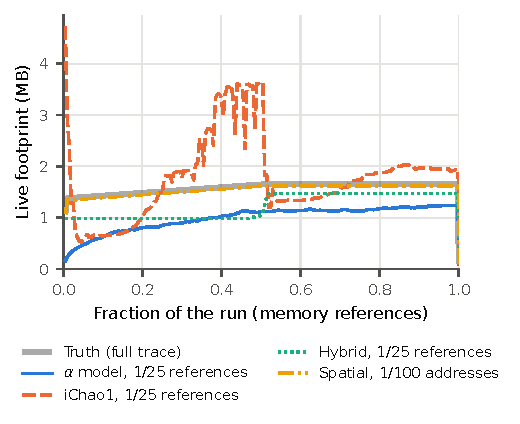
\includegraphics[width=0.55\linewidth]{figures/reference_vs_spatial.pdf}
\caption{Live footprint of 2mm MEDIUM (held out from training) over the run, against estimates from 1-in-25 samples of references and from a 1-in-100 sample of words. The word sample follows the truth closely, whereas the estimates from sampled references overshoot, undershoot or lag.}
\label{fig:reference}
\end{figure}

\paragraph{Forecasting.}
We also tried to predict the rest of a footprint curve from its beginning. We stretched each training input's curve in time and in size to match the observed beginning, and averaged the stretched curves with weights that decrease with how badly each one fitted. The predicted peak was within about 10\% to 20\% for interpolation but unreliable for extrapolation, and we did not pursue forecasting further.

%=====================================================================
\section{Sampling words}
\label{sec:spatial}

All the estimators of \secref{sec:reference} fail for the same reason. An address that is referenced $r$ times appears in a sample of references with probability $1 - (1-p)^r$, which depends on $r$, and $r$ is unknown and grows with the input size. Sampling memory instead of references removes that dependence, because a byte is then in the sample with a probability that does not depend on how often it is used.

\subsection{Method}

In the tool's \term{spatial} mode (\knob{mode spatial}), an aligned 8-byte word $w = \lfloor a/8 \rfloor$ is \term{selected} when $h(w \oplus \sigma) < 2^{64}/i$. Here $\oplus$ is the bitwise exclusive or, $\sigma$ is a 64-bit number (a salt) derived from the run's random seed, and $h$ is the final mixing function of the splitmix64 random number generator~\cite{steele2014splitmix}, which scrambles the bits of its input so that nearby words, or words at regular distances, give unrelated results. For every reference that covers a selected word, the tool records the bytes of the reference that lie inside selected words.

Each byte is selected with probability $1/i$, independently of how the program uses it. Let $F_S(t)$ be the number of selected bytes touched and live at time $t$. Every byte of the true footprint contributes to $F_S$ with probability $1/i$, so the expected value of $F_S(t)$ is $F(t)/i$, and
\begin{equation}
\hat{F}(t) = i\,F_S(t)
\end{equation}
is an \term{unbiased} estimate of $F(t)$, meaning that its average over many choices of the salt equals the truth. It is the Horvitz--Thompson estimator~\cite{horvitz1952} for a sample in which every element has the same probability of being included~\cite{cochran1977}. No model and no training are needed. The number of selected words follows a binomial distribution, so for $U$ touched words, the standard deviation of the estimate relative to the truth is about $\sqrt{(1 - 1/i)\,i/U} \approx 1/\sqrt{U/i}$. For example, 200{,}000 words sampled at 1 in 100 give about 2\%.

The unit matters. A first version selected 64-byte chunks, which is 8 times fewer units for the same memory, and its error on PolyBench was about $\sqrt{8} \approx 2.8$ times larger (7.4\% instead of 2.8\% at 1 in 100 on the largest inputs). With the start-address footprint the unit is the start address, which for 8-byte numbers gives the same precision as words.

To report an error bar, the tool also splits the selected words into 20 \term{buckets} by the value of $h(w \oplus \sigma) \bmod 20$. Each bucket is an independent 1-in-$20i$ sample, so $20\,i\,F_{\text{bucket}}$ is an independent estimate of $F$, and the standard deviation of the 20 bucket estimates divided by $\sqrt{20}$ is a standard error of $\hat{F}$.

\paragraph{Implementation.}
The selection test is an inlined test routine that receives the reference's address and size, adds one to the running thread's reference counter, and returns whether any word the reference covers is selected. A reference of up to 16 bytes covers at most three words, which the inlined test checks; for wider references, whose size is known when the instruction is instrumented, a routine with a loop checks every word. A selected reference calls an action routine that records it immediately in the footprint and in its bucket, while holding a lock shared by all threads. Because selected references are rare, recording them immediately costs little, and it keeps the order of references and frees across threads exact, because the tool also applies frees immediately under the same lock. The time of a snapshot is the sum of the threads' reference counters.

We first recorded selected references through trace buffers, as the splitter does, which brought back the ordering problem of \secref{sec:ordering}. We then held each free back until every thread had processed all the references it had made before the free, using vector clocks, which record for each thread how many events of every other thread it has seen. This approach was correct, but miniVite frees memory constantly while its MPI helper threads rarely fill a buffer, so a run at 8192 vertices took 7474\,s. Recording selected references immediately took 28 to 40\,s for the same run, and the 8-thread test of \secref{sec:ordering} then gives 12.03 to 12.27\,MB, against a truth of 12.09\,MB.

\subsection{Results}

\paragraph{PolyBench.}
With the largest and middle of the sizes MINI to MEDIUM held out, as in \secref{sec:reference}, word sampling has 1.6\% and 4.0\% mean error at 1 in 25 words, 2.8\% and 4.9\% at 1 in 100, 2.9\% and 4.1\% at 1 in 250, and 5.3\% and 16.0\% at 1 in 1000 (\figref{fig:spatial}). The error follows the binomial prediction. The largest sizes (130{,}000 to 200{,}000 words) stay within about 5\% down to 1 in 1000, whereas the middle sizes (about 28{,}000 words) need 1 in 250 or denser, because at 1 in 1000 only about 28 of their words are selected. For the largest sizes, the true footprint lies within two standard errors of the estimate in 99\% of snapshots at 1 in 25 and 1 in 100 and in 75\% at 1 in 250, against 95\% expected, because a standard error computed from 20 buckets is itself uncertain.

\paragraph{miniVite and threads.}
With frees tracked, the live peak of miniVite is 3.8, 4.8 and 6.3\,MB at 1024, 4096 and 8192 vertices, the same at every thread count. Word sampling has 0.3\% to 6.8\% mean error at every rate from 1 in 25 to 1 in 1000 with 1, 4 and 16 threads, and the error of the peak is at most 3.6\% at 1 in 100 or denser and at most 7.7\% at 1 in 1000. The error bars are less reliable than on PolyBench: the truth lies within two standard errors in 98\% to 100\% of snapshots in most runs, but in only 1\% to 69\% in a few runs, which are off by more than their buckets suggest. At 8192 vertices a run takes 25 to 41\,s, against 175 to 187\,s for a complete recording and 0.16 to 0.22\,s natively.

\paragraph{Cost on large inputs.}
On the LARGE PolyBench inputs, word sampling at 1 in 100 takes 284\,s for 2mm, 271\,s for gemm and 344\,s for jacobi-2d, against 8.0, 5.1 and 11.3\,s natively, which is an overhead of 30$\times$ to 53$\times$. Pin without a tool takes 8.2, 5.4 and 11.5\,s, so almost all of the cost is the selection test on every reference. The test checks one or two words for most references, against one start address for the start-address footprint, which took 211 to 236\,s.

\begin{figure}[t]
\centering
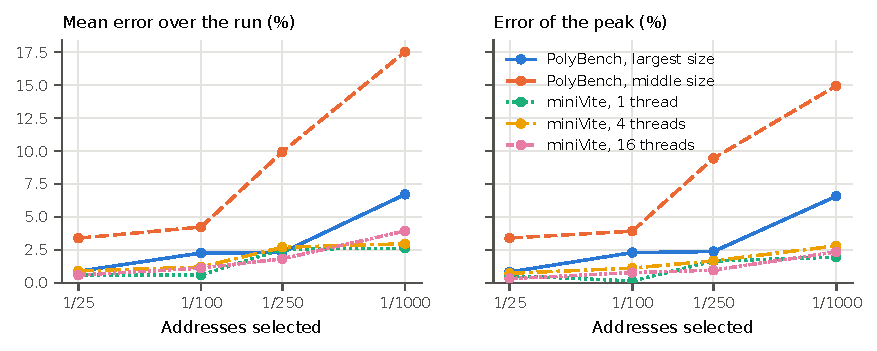
\includegraphics[width=\linewidth]{figures/spatial_rate.pdf}
\caption{Word sampling error against the fraction of words selected. PolyBench values are the mean over 2mm, gemm, jacobi-2d and atax for the held-out largest and middle of the sizes MINI to MEDIUM. miniVite values are the mean over 1024, 4096 and 8192 vertices.}
\label{fig:spatial}
\end{figure}

%=====================================================================
\section{Windowed sampling}
\label{sec:windowed}

Word sampling still runs the selection test on every reference, which costs 30$\times$ to 53$\times$ native time on the LARGE PolyBench inputs, whereas Pin without a tool costs almost nothing. For long programs, therefore, the test itself is the obstacle, not the sampling rate. \term{Windowed sampling} (options \knob{window W} and \knob{period P}) runs the selection test only during \term{windows} of $W$ references at the start of every $P$ references, so that a fraction $W/P$ of the run is \term{watched}. Between windows it runs only things that cost little and that still observe the whole run. \figref{fig:design} gives an overview, and the rest of this section describes each part.

\begin{figure}[t]
\centering
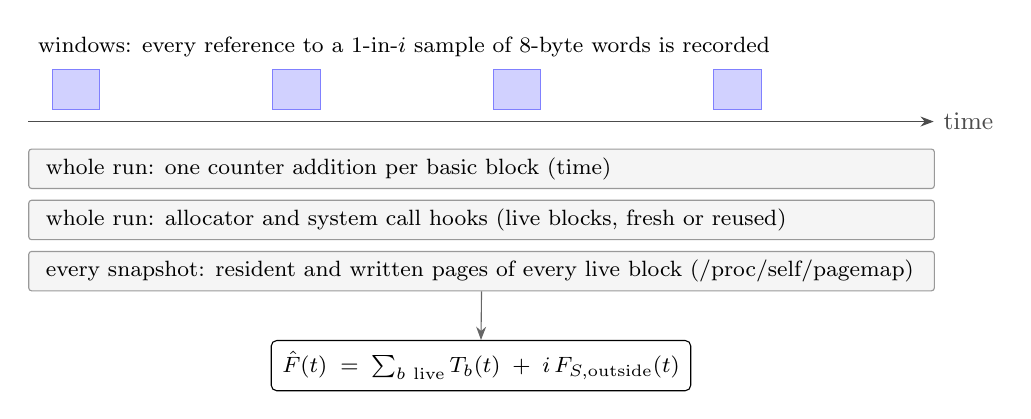
\begin{tikzpicture}[font=\small, >=Stealth,
  lane/.style={draw=black!40, rounded corners=1pt, minimum height=5mm, inner sep=2pt},
  win/.style={fill=blue!18, draw=blue!50, minimum height=5mm, inner sep=0pt}]
  \def\L{11.5}
  \draw[->, black!70] (0,0) -- (\L,0) node[right] {time};
  \foreach \x in {0.3, 3.1, 5.9, 8.7} {
    \node[win, minimum width=6mm, anchor=south west] at (\x,0.15) {};
  }
  \node[anchor=west, font=\footnotesize] at (0,0.95) {windows: every reference to a 1-in-$i$ sample of 8-byte words is recorded};
  \node[lane, minimum width=\L cm, anchor=west, fill=black!4] at (0,-0.6) {};
  \node[anchor=west, font=\footnotesize] at (0.1,-0.6) {whole run: one counter addition per basic block (time)};
  \node[lane, minimum width=\L cm, anchor=west, fill=black!4] at (0,-1.25) {};
  \node[anchor=west, font=\footnotesize] at (0.1,-1.25) {whole run: allocator and system call hooks (live blocks, fresh or reused)};
  \node[lane, minimum width=\L cm, anchor=west, fill=black!4] (res) at (0,-1.9) {};
  \node[anchor=west, font=\footnotesize] at (0.1,-1.9) {every snapshot: resident and written pages of every live block (/proc/self/pagemap)};
  \node[draw, rounded corners=2pt, align=center, font=\footnotesize, inner sep=4pt] (est) at (\L/2,-3.1)
    {$\hat F(t) \;=\; \sum_{b\ \text{live}} T_b(t) \;+\; i\,F_{S,\text{outside}}(t)$};
  \draw[->, black!60] (res.south) -- (est.north);
\end{tikzpicture}
\caption{Windowed sampling. References are checked only inside windows (shaded). Time, live blocks and page information are tracked for the whole run. $T_b$ is the touched bytes of block $b$ (resident bytes for a fresh block, bytes on written pages for a reused block), and $F_{S,\text{outside}}$ is the selected bytes outside all blocks.}
\label{fig:design}
\end{figure}

\subsection{Counting time between windows}
\label{sec:counting}

Between windows the tool must still count references, because time is measured in references, and windows start and end at given times. Counting each reference separately would cost almost as much as the selection test. Instead, when Pin translates a basic block, the tool counts the block's memory references, which is the number of memory operands that the block's instructions read plus the number that they write, and it inserts one inlined call at the start of the block that adds that number to the running thread's counter. The same call compares the counter with a threshold and, only when the threshold is reached, calls a longer routine that advances time for all threads (\secref{sec:switching}).

On miniVite with one thread, this count matches the splitter's count of every reference to within 0.0001\% over 1.78 billion references. The two counts differ in two cases. An instruction with a REP prefix, which repeats a string operation many times, counts once rather than once per repetition, and a basic block that is left before its end, for example because of a signal, still counts all its references.

Each thread's counter sits in its own 64-byte memory area, which is the unit in which processors cache memory, so that threads do not slow each other down by writing into the same cached unit.

\subsection{Switching between watching and not watching}
\label{sec:switching}

When a thread's counter passes its threshold, the thread takes the shared lock, adds up all threads' counters to get the current time, writes any snapshot that is due, and opens or closes a window if the time has passed a window's start or end. It then sets its next threshold $s$ references ahead, where
\begin{equation}
s = \max\!\left(10^4,\; \tfrac{1}{8}\min(W,\; P - W,\; N)\right),
\end{equation}
so that every thread checks the time several times within the shortest of a window, a gap between windows and a snapshot interval, but not so often that the lock becomes expensive. The first version used $10^3$ instead of $10^4$, and a run with 1000-reference windows then spent most of its time taking the lock.

When a window opens or closes, the instrumentation must change, because inside a window every reference needs the selection test, and outside a window it does not. The tool calls \texttt{PIN\_RemoveInstrumentation}, after releasing the lock, which discards all translations, so that Pin translates code again, with the new instrumentation, the next time it runs. However, discarding translations does not change code that is already running. A loop keeps jumping back to the start of its own translation, so it keeps running the old instrumentation until it leaves the loop. In 2mm, a window that had closed kept the selection test running for the rest of a loop nest, so a run that should have watched almost nothing took 70\,s instead of 19\,s, and windows did not start or stop on time.

The tool therefore counts window changes in a shared counter, and each thread remembers the last change it has acted on. When a thread checks the time and finds a change it has not acted on, it restarts at its current instruction with \texttt{PIN\_ExecuteAt}, using the machine state that Pin passes to the routine, so that Pin translates the code it is running again. Threads check the time every $s$ references also while running old code, because the counting call is present in both versions of the code. A reference that old code records after a window has closed is discarded.

Discarding all translations has a cost that grows with the amount of code a program runs. For most programs it is small, but GCC's compiler runs a lot of code, and with 20 windows, which is 40 changes, it took 658 to 963\,s, against 101 to 122\,s with nothing watched and 182\,s watching the whole run (\secref{sec:cost}).

\subsection{Tracking live blocks}
\label{sec:blocks}

In windowed mode the allocator hooks of \secref{sec:frees} are always on, and the tool keeps every live block in an ordered map from start address to size, so that it can find the block that contains a given address. It also records memory that the program maps directly. When an \texttt{mmap} system call that maps anonymous memory succeeds outside an allocation call, the tool adds the mapping as a block, and when \texttt{munmap} unmaps part of such a block, the tool removes that part and keeps the rest. When \texttt{realloc} grows or shrinks a block in place, the tool keeps the block and changes its size.

The tool classifies each block as \term{fresh} or \term{reused}. A block is fresh when its pages were mapped for it, which is the case for an anonymous mapping made outside the allocator, and for an allocation during which the allocator called \texttt{mmap} or \texttt{mremap}. The tool knows the latter because it watches system calls and knows which thread is inside an allocation call. By default, the GNU C allocator serves requests of 128\,KB or more by mapping new memory~\cite{glibcmanual}, so large arrays are usually fresh. All other blocks are reused, because the allocator takes them from memory it already owns, which may have been used by blocks that were freed earlier.

\subsection{Page residency}
\label{sec:residency}

A fresh block's pages are untouched when the block is created, and a page becomes resident at its first read or write. The number of a fresh block's bytes that lie on resident pages is therefore the number of bytes the block has touched, rounded to whole pages, whether or not a window is open.

The tool reads residency from \texttt{/proc/self/pagemap}~\cite{pagemap}, a file through which Linux reports one 64-bit entry per page of the process. In an entry, bit 63 is set if the page is resident, bit 62 if it has been moved to swap space, and bit 55 if it has been written since the last reset of that bit (\secref{sec:written}). At every snapshot the tool visits the live blocks in address order, reads the entries of their pages in chunks of 512 pages so that neighboring blocks share reads, and for each block adds up the bytes of the block that lie on resident or swapped pages. At a block's first and last page it counts only the bytes inside the block. Pin's C library does not provide the \texttt{pread} function, so the tool uses \texttt{lseek} followed by \texttt{read}.

Our machine enables transparent huge pages~\cite{thp}, which let the operating system back a 2\,MB region with one large page at its first touch. A single touch can then make a whole 2\,MB region resident. In a test that wrote 16\,MB of a 64\,MB block, pagemap reported 18.4\,MB resident with huge pages on. The tool therefore turns off huge pages for the traced process with \texttt{prctl(PR\_SET\_THP\_DISABLE)}, through the raw system call because Pin's C library does not provide \texttt{prctl}. With huge pages off, the same test reports exactly 16\,MB, and reading another 8\,MB adds exactly 8\,MB, because a read of untouched memory also makes its page resident.

\subsection{Written pages of reused blocks}
\label{sec:written}

The residency of a reused block can include pages that earlier blocks at the same addresses touched, because memory that a program frees stays resident and the allocator hands it to later blocks. In a test that keeps 64 heap blocks live, replaces the oldest one at every step, and writes only the first quarter of each new block (\secref{sec:churn-eval}), residency overestimates the live footprint by 249\%.

The tool therefore measures a reused block by the pages written since the block was allocated, using the kernel's soft-dirty bits~\cite{softdirty}. Writing the character \texttt{4} to the file \texttt{/proc/self/clear\_refs} clears the soft-dirty bit of every page of the process, and after that, bit 55 of a page's pagemap entry is set if the page has been written. Memory that the allocator returns is not initialized, so a program writes heap memory before it reads it, and the pages a reused block has written since its allocation are the pages it has touched. Each reused block keeps one mark per page, and at every snapshot the tool sets the mark of each of its pages whose soft-dirty bit is set. The touched bytes of a reused block are its bytes on marked pages.

To clear the soft-dirty bits, the kernel removes write permission from every page, so the next write to each page causes a fault, in which the kernel sets the bit and restores the permission. Each clear therefore costs one fault for each page that is written afterwards, and the tool clears the bits only at three kinds of events. Before every clear, it first sets the marks of every live reused block from the current bits, so that no write is lost.
\begin{enumerate}
\item At the entry of an allocation call of 16\,KB or more. Bits that earlier blocks set on the new block's pages are then cleared before the block exists. The clear happens at the entry rather than at the exit because \texttt{calloc} sets the new memory to zero and \texttt{realloc} copies the old block's contents inside the call, and those writes belong to the new block. Smaller blocks share pages with other blocks, so clearing for them would add cost without making their measurement exact.
\item Around the \texttt{brk}, \texttt{mmap} and \texttt{mremap} system calls. When the kernel creates or grows a memory region, it marks the whole region as soft-dirty, so that all its pages read as written until the next clear, whether or not they were written. The allocator grows the heap with \texttt{brk}, and before we handled this case, the written bytes of the churn test jumped between 1.3\,MB and 3.7\,MB from one snapshot to the next. The tool now sets the marks at the system call's entry and clears the bits at its exit.
\item Every \knob{dirty\_every} references, by default every ten snapshots.
\end{enumerate}
A block whose pages are all marked cannot change any more, so the tool skips it when it sets marks before a clear. On miniVite with one thread, which clears the bits 8509 times, this reduced the running time from 138\,s to 86\,s.

\subsection{Word sampling inside windows}
\label{sec:density}

Inside windows the tool selects 1 in $i$ words, as in \secref{sec:spatial}. The windows see memory outside every block, which covers the stack, global variables and memory mapped from files, and which pages cannot attribute to a block.

\paragraph{Density, under the start-address footprint.}
With the start-address footprint, residency and written pages measure bytes, but the footprint counts overlapping accesses more than once, so the tool multiplied each block's touched bytes by a \term{density}, the footprint divided by the bytes covered. Windows then selected 64-byte chunks, so that they saw, for some part of each block, both the footprint and the bytes covered, and a block's density was measured once its chunks covered $64\,\text{KB}/i$; otherwise a reused block used the density of all reused blocks and a fresh block used 1. In miniVite's reused blocks the density was about 1.45 for most of the run. This was the weakest part of the estimate. A block's density accumulates over a run, because every new access pattern, another width or another offset, adds start addresses to memory already covered, so a window measures a lower density than the whole run has: on GAP breadth-first search, 1.02 at 1\% watched, 1.08 at 5\% and 1.19 at 20\%, against 1.36 over the whole run, which left its peak 26\% too low at 5\% watched. With bytes touched there is no density, which is the second reason we changed the definition.

\subsection{The estimate}
\label{sec:estimate}

At every snapshot the tool writes one row to a separate output file (Appendix~\ref{app:outputs}), which includes the estimate
\begin{equation}
\hat{F}(t) = \sum_{b\ \text{live}} T_b(t) + i\,F_{S,\text{outside}}(t),
\label{eq:windowed}
\end{equation}
where $T_b$ is the touched bytes of block $b$ (resident bytes for a fresh block, bytes on written pages for a reused block), and $F_{S,\text{outside}}$ is the number of selected bytes outside every block, which only windows see. The row also contains every part of the estimate, so that other combinations can be evaluated without running the program again.

\subsection{Windows opened by large allocations}
\label{sec:allocwindows}

With \knob{window\_alloc N} (by default 1\,MB), an allocation of at least $N$ bytes also opens a window at once, at most one per period on top of the periodic windows, so that at most twice the periodic fraction is watched. A large allocation is usually followed by the program filling the block, and with the start-address footprint a window opened then measured the block's density. A periodic window that starts inside such a window extends it.

With the start-address footprint these windows mattered. On miniVite with 65536 vertices, a 25\,MB fresh block allocated at 88\% of the run was inside no periodic window and counted with density 1.00 instead of 1.28, while a 9\,MB reused block allocated at 94\% took the density of the other reused blocks, 1.44 instead of 1.00; the two errors cancelled at the peak ($-2.6\%$). Windows opened at both allocations measured both blocks exactly. With bytes touched there is no density to measure, and these windows change the error by less than one point (\secref{sec:windowed-eval}).

\subsection{Approaches that did not work}
\label{sec:history}

We arrived at \eqref{eq:windowed} after several approaches that failed, which we list in the order in which we tried them.
\begin{enumerate}
\item \textbf{The windows' sample alone.} Multiplying the selected bytes by $i$ misses every address that is touched only between windows. On 2mm LARGE at 1\% watched it has 47\% mean error.
\item \textbf{A model per allocation site.} We estimated a block from the selected bytes that windows had seen in it, and a block that no window had yet seen from the fraction touched in earlier blocks allocated at the same place in the program. This estimate also missed every touch made between windows, and it had 29\% to 47\% mean error on miniVite at 1\% watched and 8\% to 25\% at 5\%.
\item \textbf{Residency for all blocks.} Residency is exact for fresh blocks but overestimates reused blocks that sit on memory used before, by 249\% on the churn test.
\item \textbf{A density from sampled pages.} Dividing the selected footprint by the resident bytes of the pages that contained a selected address was noisy, and one run ended with a density of 2.7, because a page with few touched addresses enters the calculation only when one of them is selected.
\item \textbf{Densities measured in windows.} Under the start-address footprint, one density for all reused blocks, and later one per block, left peaks up to 15\% too low on miniVite and up to 66\% too low on the programs of \secref{sec:real}, because density accumulates over the whole run (\secref{sec:density}).
\end{enumerate}

%=====================================================================
\section{Evaluation of windowed sampling}
\label{sec:windowed-eval}

We compare windowed runs with a complete recording of the same input and thread count. All runs select 1 in 100 words and use about 20 windows per run (the period is about one twentieth of the run), with periodic windows only unless we say otherwise, and we did not tune any setting for any workload. We compare \eqref{eq:windowed} with three simpler estimates: \term{residency alone}, which is the resident bytes of all blocks plus the windows' selected bytes outside blocks, without written pages; the windows' selected bytes alone ($i\,F_S$); and the bytes of all live blocks, which we call the \term{allocated bytes}.

\subsection{PolyBench}

Every PolyBench array is allocated by mapping new memory, so all blocks are fresh and residency alone gives the exact curve. The windowed estimate is within 0.0\% to 0.1\% mean error and within 0.1\% at the peak at every watched fraction, including none (\figref{fig:curves}, left). The windows' sample alone has 0.1\% to 10.9\% mean error at 5\% watched and 10.9\% to 46.7\% at 1\%, because it misses memory that is written once and then not used while a window is open. The allocated bytes have 0.4\% to 4.5\%.

\begin{figure}[t]
\centering
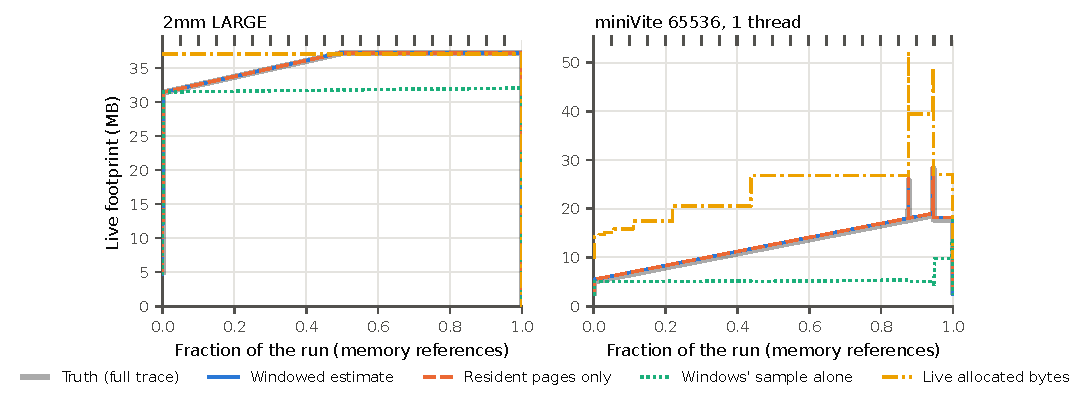
\includegraphics[width=\linewidth]{figures/windowed_curves.pdf}
\caption{Live footprint over the run with 5\% of the run watched (20 windows, marked at the top) and 1 in 100 words selected. On 2mm LARGE the windowed estimate and residency alone coincide with the truth.}
\label{fig:curves}
\end{figure}

\subsection{miniVite}

miniVite's footprint grows in reused heap blocks for the whole run, and it allocates far more than it touches, so the allocated bytes overestimate it, with 107\% to 164\% mean error (\figref{fig:curves}, right). \tabref{tab:windowed} and \figref{fig:fraction} show the windowed estimate. With 5\% watched, it has 3.3\% to 4.0\% mean error and $+1.3\%$ to $+1.8\%$ error of the peak on both inputs and both thread counts. Watching matters only for memory outside blocks, which only windows see: with nothing watched, the peak is 4\% to 7\% too low, and 1\% watched is enough. Watching more does not help, and the estimate rises by one to two points between 1\% and 20\% watched, as whole pages and selected words outside blocks accumulate. Selecting 1 in 25 words instead of 1 in 100 changes the results by less than one percentage point, and one and four threads agree within one point. Residency alone is as good as the estimate on miniVite, because its reused blocks are written all over.

With the start-address footprint, the same runs had 1.7\% to 17.1\% mean error and $-0.4\%$ to $-15.2\%$ error of the peak at 1\% to 20\% watched, and about 25\% too low a peak with nothing watched, because the density had to be measured in windows.

\begin{table}[t]
\centering
\small
\caption{Windowed estimate on miniVite, mean error / error of the peak in percent, 1 in 100 words, about 20 windows.}
\label{tab:windowed}
\begin{tabular}{lccccc}
\toprule
Input, threads & Nothing watched & 1\% & 5\% & 20\% & Everything \\
\midrule
65536 vertices, 1 thread & 10.1 / $-3.8$ & 2.8 / $+1.1$ & 3.9 / $+1.5$ & 3.7 / $+1.4$ & 3.6 / $+1.4$ \\
65536 vertices, 4 threads & 9.8 / $-3.7$ & 2.4 / $+0.9$ & 3.6 / $+1.3$ & 4.2 / $+1.6$ & 3.8 / $+1.4$ \\
32768 vertices, 1 thread & 14.7 / $-6.9$ & 1.0 / $+0.5$ & 3.3 / $+1.5$ & 5.3 / $+2.5$ & 4.9 / $+2.3$ \\
32768 vertices, 4 threads & 14.6 / $-6.9$ & 1.8 / $+0.8$ & 4.0 / $+1.8$ & 5.3 / $+2.5$ & 5.7 / $+2.7$ \\
\bottomrule
\end{tabular}
\end{table}

\begin{figure}[t]
\centering
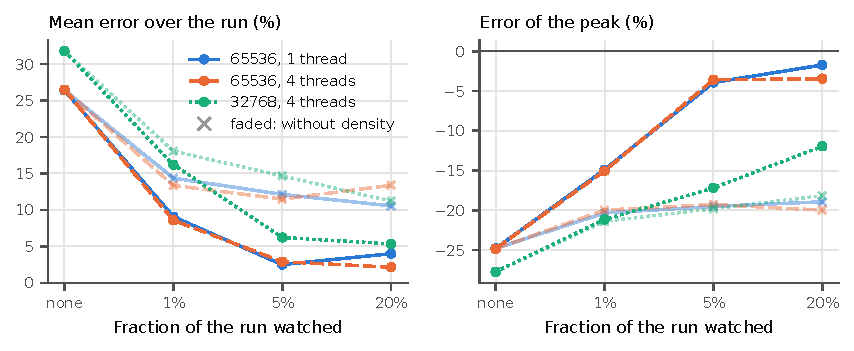
\includegraphics[width=\linewidth]{figures/windowed_fraction.pdf}
\caption{miniVite: windowed estimate error against the fraction of the run watched, with 1 in 100 words. Faded lines are residency alone, without written pages.}
\label{fig:fraction}
\end{figure}

\paragraph{Windows opened by large allocations.}
miniVite makes 5 to 7 allocations of 1\,MB or more that open windows. With them the results change by about one point or less (for example 3.6\% / $+1.4\%$ instead of 3.9\% / $+1.5\%$ at 5\% watched with one thread on 65536 vertices). PolyBench and the churn test open no such windows.

\subsection{Heap churn}
\label{sec:churn-eval}

The heap-churn test keeps 64 live heap blocks of 16 to 112\,KB, which is below the allocator's threshold for mapping new memory, so all blocks come from memory that the allocator reuses. At every step it frees the oldest block, allocates a new one, writes the first quarter (or half) of the new block, and reads the written part of one other live block. Its live footprint peaks at 1.3\,MB when a quarter of each block is written and at 2.5\,MB when half is written.

Residency alone overestimates the footprint by 249\% (mean error) when a quarter of each block is written and by 91\% when half is written, because the pages of freed blocks stay resident and are handed to new blocks (\figref{fig:churn}). Measuring reused blocks by their written pages reduces the error to 24\% and 13\%. The error is about the same at every watched fraction (23\% to 26\% when a quarter is written), because written pages, not windows, carry the estimate. The remaining error comes from whole pages. Each block's written part ends inside a 4\,KB page, which adds up to 4\,KB per block, or about 0.25\,MB for 64 blocks.

\begin{figure}[t]
\centering
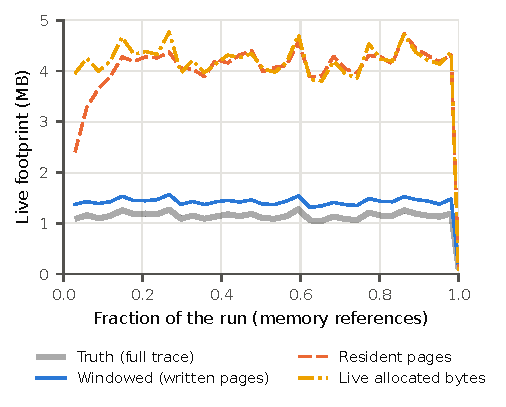
\includegraphics[width=0.55\linewidth]{figures/churn.pdf}
\caption{Heap churn with a quarter of each block written, 5\% of the run watched. Resident pages include memory that freed blocks touched, whereas the pages written since each block's allocation follow the truth to within whole pages.}
\label{fig:churn}
\end{figure}

\subsection{Programs that reuse their heap}
\label{sec:real}

\tabref{tab:real} shows the windowed estimate on the GAP kernels, darknet, the interpreters, SQLite and GCC, with allocation windows on. Lua, Perl and SQLite keep 84\% to 100\% of their live memory in reused heap blocks (44 to 73\,MB at the peak, in 24{,}000 to 650{,}000 blocks), whereas GAP, darknet, Python and GCC keep most of theirs in fresh blocks: GAP's and darknet's arrays are large, Python's small-object allocator takes 256\,KB regions from the operating system, and GCC's garbage collector maps its pages. In every program, the residency of the reused blocks exceeds their written pages by at most 1.2\,MB at any point: the blocks are reused, but each new block is written all over. Forcing large blocks of GAP and darknet onto the heap, with the environment variable \texttt{MALLOC\_MMAP\_THRESHOLD\_}, moved 5 to 86\,MB into reused blocks, and residency still exceeded the written pages by at most 1\,MB.

Every peak is within $-5.4\%$ to $+6.7\%$ at every watched fraction, including none. The programs that touch what they allocate (GAP, Lua, Perl, SQLite) are estimated almost as well by their allocated bytes, at the peak; darknet, which touches half of what it allocates, is not ($+97\%$). On GCC and Lua, watching moves the peak up by three to ten points, as the windows' selected bytes outside blocks exceed what is live there; we have not found which memory that is. With the start-address footprint, the peaks of the same programs were 5\% to 66\% too low at 5\% watched, mostly because of density, and also because the truth then counted the allocator's bookkeeping (\secref{sec:allocator}).

\begin{table}[t]
\centering
\small
\caption{Windowed estimate on programs that reuse their heap, mean error / error of the peak in percent, 1 in 100 words, allocation windows on. Single thread unless stated.}
\label{tab:real}
\begin{tabular}{lrccccc}
\toprule
Program & True peak & Allocated bytes & Nothing & 1\% & 5\% & Everything \\
\midrule
GAP bfs & 72.8\,MB & 201.9 / $-0.3$ & 5.0 / $-0.3$ & 3.1 / $-0.0$ & 2.1 / $+0.2$ & 2.3 / $+0.2$ \\
GAP pr & 72.5\,MB & 143.8 / $-0.0$ & 3.8 / $-0.0$ & 1.8 / $+0.4$ & 1.7 / $+0.5$ & 1.5 / $+0.5$ \\
GAP cc & 72.8\,MB & 198.7 / $-0.3$ & 4.9 / $-0.3$ & 3.0 / $-0.0$ & 1.9 / $+0.1$ & 2.0 / $+0.2$ \\
GAP sssp & 133.8\,MB & 183.3 / $+1.3$ & 3.6 / $-0.2$ & 2.4 / $+0.1$ & 2.3 / $+0.1$ & 2.3 / $+0.0$ \\
GAP pr, 4 threads & 72.6\,MB & 337.6 / $+34.6$ & 8.3 / $-0.0$ & 11.7 / $+0.4$ & 6.4 / $+0.5$ & 4.1 / $+0.5$ \\
darknet & 269.9\,MB & 153.2 / $+96.9$ & 3.1 / $+4.0$ & 3.2 / $+4.6$ & 3.2 / $+4.1$ & 3.2 / $+4.1$ \\
Python & 95.7\,MB & 3.4 / $+3.0$ & 3.4 / $+2.8$ & 4.1 / $+3.8$ & 3.5 / $+3.8$ & 4.9 / $+4.0$ \\
Lua & 55.5\,MB & 5.8 / $-5.6$ & 5.9 / $-5.4$ & 6.6 / $-4.8$ & 6.2 / $-3.7$ & 11.8 / $+5.2$ \\
Perl & 54.9\,MB & 1.7 / $-2.3$ & 1.9 / $-3.5$ & 1.9 / $-2.9$ & 1.9 / $-2.7$ & 1.7 / $-0.6$ \\
SQLite & 76.2\,MB & 16.9 / $-2.9$ & 6.4 / $-0.7$ & 8.5 / $-2.4$ & 8.2 / $-2.5$ & 8.4 / $-0.8$ \\
GCC \texttt{cc1} & 105.4\,MB & 11.5 / $+8.3$ & 3.6 / $+3.5$ & 8.1 / $+6.4$ & 8.5 / $+6.7$ & 8.9 / $+6.6$ \\
\bottomrule
\end{tabular}
\end{table}

\subsection{Cost}
\label{sec:cost}

\tabref{tab:cost} and \figref{fig:cost} report running times measured one at a time on an otherwise idle machine, one run per configuration, except where a run was repeated (the table then shows the median). On PolyBench LARGE, windowed sampling at 5\% watched costs 3.5$\times$ (jacobi-2d) and 3.6$\times$ (2mm) native time, and 4.5$\times$ to 12$\times$ on gemm, whose running time varied between 23 and 61\,s over three runs (the table shows the median), against 30$\times$ to 53$\times$ for word sampling of every reference, and with nothing watched it costs 1.9$\times$ to 2.3$\times$, which is mostly the cost of the per-block counter. Each further percent watched adds about 0.8\% of the cost of word sampling over that floor. On miniVite with 65536 vertices it costs 14.9$\times$ with one thread and 18.1$\times$ with four at 5\% watched, against 34$\times$ and 37$\times$ for word sampling, and 12.6$\times$ and 16.7$\times$ at 1\%, which is as accurate.

The cost on miniVite is higher for three reasons. First, Pin itself costs about 1.8$\times$, because Pin translates the MPI library's start-up code once and the run is short. Second, miniVite makes 8 million \texttt{malloc} and \texttt{free} calls at 65536 vertices, each of which runs the allocator hooks and takes the lock, and on miniVite with 16384 vertices, turning the allocator hooks off saved 7\,s of 22\,s. Third, soft-dirty tracking cost about 14\% at 5\% watched in an earlier measurement, and 4\% to 14\% on PolyBench. The complete recordings that provided the truth took 3116 to 4080\,s, but they ran at the same time as other runs, so they are not directly comparable.

On the programs of \tabref{tab:real}, measured with several runs at once and therefore only roughly, Python, Lua, Perl and SQLite took 24 to 91\,s with nothing watched, 52 to 216\,s at 5\% watched and 95 to 364\,s watching everything, against 450 to 1684\,s for their complete recordings. GCC took 101 to 122\,s with nothing watched and 182\,s watching everything, but 658 to 963\,s with windows, because every window change makes Pin translate all of its code again (\secref{sec:switching}).

\begin{table}[t]
\centering
\small
\caption{Running time in seconds, one run each, 1 in 100 words, about 20 windows.}
\label{tab:cost}
\begin{tabular}{lrrrrrrr}
\toprule
& & Pin, & Word & \multicolumn{4}{c}{Windowed, fraction watched} \\
\cmidrule(lr){5-8}
Workload & Native & no tool & sampling & none & 1\% & 5\% & 20\% \\
\midrule
2mm LARGE & 8.0 & 8.2 & 284 & 15.7 & 18.1 & 29.0 & 67.7 \\
gemm LARGE & 5.1 & 5.4 & 271 & 11.5 & 13.9 & 48.1 & 56.6 \\
jacobi-2d LARGE & 11.3 & 11.5 & 344 & 21.6 & 25.0 & 39.8 & 93.3 \\
miniVite 65536, 1 thread & 6.4 & 11.7 & 216 & 67.4 & 81.2 & 96.1 & 121 \\
miniVite 65536, 4 threads & 6.0 & 11.1 & 221 & 84.1 & 101 & 109 & 136 \\
\bottomrule
\end{tabular}
\end{table}

\begin{figure}[t]
\centering
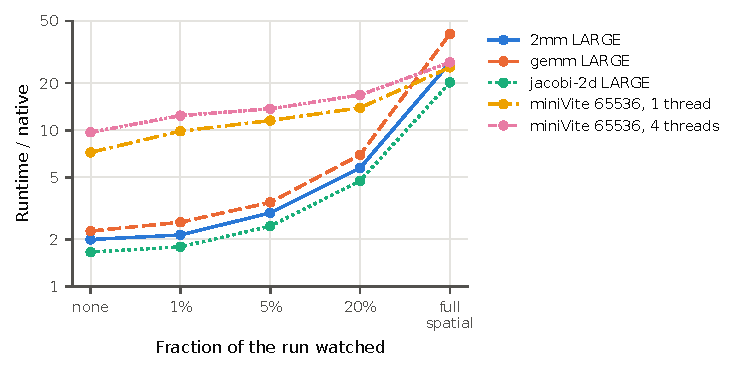
\includegraphics[width=0.75\linewidth]{figures/cost.pdf}
\caption{Running time relative to native time against the fraction of the run watched, with word sampling of every reference for comparison (logarithmic scale).}
\label{fig:cost}
\end{figure}

%=====================================================================
\section{Discussion and limitations}
\label{sec:discussion}

\paragraph{Why each part is needed.}
Each part of \eqref{eq:windowed} corrects one failure that we observed. Residency records first touches whether or not a window is open, which the windows' sample alone cannot do. Written pages remove the pages that a reused block inherits from freed blocks, which residency alone cannot do. The windows see memory outside every block, which pages cannot attribute. With bytes touched, that is all: the density, which was the weakest part of the estimate, is gone, and with it most of the reason to watch more than 1\% of a run.

\paragraph{The definition of the footprint.}
The start-address footprint of \memprint{} measures the access pattern as well as the memory, by up to 3.4$\times$ on SQLite, and a heap profiler measures allocation, which can be 2$\times$ to 4$\times$ the memory touched. The bytes touched are bounded by the resident memory, which our validation confirmed on every workload. The tool keeps the start-address footprint for \memprint{}'s whole-run model, whose outputs do not change.

\paragraph{Limitations of written pages.}
A limitation of written pages is that they miss memory that a reused block only reads, which is rare for heap memory because the allocator does not initialize it, and that they are exact only to the page, which adds up to 4\,KB per block and dominates for programs with many small blocks that are only partly touched (23\% on the churn test). Pages also round up fresh blocks that are touched only in part, which is darknet's $+4\%$. Blocks smaller than 16\,KB do not clear the soft-dirty bits when they are allocated, so they can inherit marks from writes made since the last clear. With several threads, writes that other threads make between the entry and the exit of a \texttt{brk} or \texttt{mmap} call are cleared without being recorded.

\paragraph{Limitations of the allocator handling.}
The tool recognizes the GNU C library's allocator by the names of its functions, which needs the library's symbol table, and it reads the allocator's chunk size field to release a whole chunk. Programs that use another allocator, such as jemalloc or tcmalloc, or that manage memory inside large regions of their own, as Python's small-object allocator and GCC's garbage collector do, are tracked only at the level of the regions that they map.

\paragraph{Other limitations.}
Memory outside blocks, such as the stack and global variables, is seen only in windows. The tool does not track \texttt{mremap} calls made outside \texttt{realloc}, \texttt{madvise}, or the growth and shrinking of the stack. Every window change discards all translated code, which is expensive for programs with a lot of code. Address and word selection depend on absolute addresses, which move when the tool library changes size, because the operating system places the program's mappings around the tool's, so spatial and windowed outputs are not byte for byte identical across builds of the tool, whereas splitter and sampler outputs are. Soft-dirty tracking requires a Linux kernel built with soft-dirty support, and the tool falls back to residency for reused blocks if \texttt{/proc/self/clear\_refs} cannot be written.

\paragraph{Generality of the evaluation.}
We evaluated two scientific applications, four graph kernels, a neural network, three interpreters, a database, a compiler and one synthetic test, each on one input. It remains unclear how the windowed estimate behaves on long programs whose footprint changes in phases shorter than a window period, and with many MPI processes.

%=====================================================================
\section{Related work}
\label{sec:related}

\paragraph{Measuring memory use.}
Valgrind~\cite{Nethercote2007Valgrind} is a binary instrumentation framework, and its heap profilers Massif~\cite{ValgrindMassif} and DHAT~\cite{dhat} record every allocation and report the amount of heap memory reserved over time, at a high cost and without measuring which reserved bytes are used; DHAT also counts the accesses to each byte offset of small blocks. Pin~\cite{Luk2005Pin} and DynamoRIO~\cite{bruening2003dynamorio} are binary instrumentation frameworks on which tools that record every memory access can be built, as \memprint{}~\cite{memprint} does. The working set model~\cite{denning1968} defines the memory that a program needs as the pages it used during a recent interval of time, which is a page-level, time-limited counterpart of the live footprint.

\paragraph{Hardware sampling of memory accesses.}
Intel's Processor Event-Based Sampling (PEBS) and ARM's Statistical Profiling Extension (SPE) let the processor record the address of a sampled memory access at low cost~\cite{roca_nonell2020pebs,miksits2024arm_memprof}. MemGaze~\cite{Xu2020MemGaze} analyzes traces of sampled loads, and HeMem~\cite{raybuck2021hemem} uses PEBS to decide which pages to place in fast memory. These approaches sample accesses, as the \memprint{} sampler does, so an estimate of the footprint from them faces the bias of \secref{sec:reference}: frequently used memory is far more likely to be seen.

\paragraph{Page-level tracking by the operating system.}
Thermostat~\cite{agarwal2017thermostat} samples pages and observes accesses to them by changing their page table entries, and DAMON~\cite{park2019damon} monitors how often memory regions are accessed in the Linux kernel by checking the accessed bits of sampled pages. Linux reports residency through \texttt{/proc/pid/pagemap}~\cite{pagemap} and written pages through soft-dirty bits~\cite{softdirty}, which tools that save and restore processes use to find the pages changed since a previous save. We use residency and soft-dirty bits to measure first touches between windows, to the page, and we use sampled references to see what pages cannot attribute.

\paragraph{Sampling locations in caches and simulation.}
Simulating only a subset of cache sets, or only the addresses chosen by a hash, is an established way to make cache simulation cheaper~\cite{kessler1994}. SHARDS~\cite{waldspurger2015shards} keeps the references whose address hashes below a threshold to build miss ratio curves for storage caches from a small fixed fraction of the addresses, which is the same selection as our word sampling. Counter stacks~\cite{wires2014counterstacks} use probabilistic counters to estimate distinct elements and miss ratio curves for storage traces. Reuse distance analysis~\cite{mattson1970,Beyls2005ReuseDistance}, StatCache~\cite{Berg2013StatCache} and StatStack~\cite{eklov2010statstack} estimate cache behavior from sampled reuse, rather than the footprint over time.

\paragraph{Sampling over time.}
PinPoints~\cite{patil2005pinpoints} and SimPoint~\cite{sherwood2002simpoint} choose representative regions of a run, SMARTS~\cite{wunderlich2003smarts} simulates many short, regularly spaced samples of a run in detail, and instrumentation sampling for datacenter applications~\cite{cho2013instrumentation} turns instrumentation on and off over time, as our windows do. These methods estimate quantities that each region shows by itself, such as instructions per cycle. A footprint depends on the first touch of every address, which can happen outside every sampled region, which is why windowed sampling needs residency and written pages between windows.

\paragraph{Estimating unseen elements.}
Good~\cite{good1953} introduced the estimation of the probability of unseen species from frequency counts, and Chao1~\cite{chao1984} and iChao1~\cite{chiu2014ichao} estimate the number of unseen species~\cite{bunge1993}. Our known-rate estimator adapts these ideas to a sample whose rate is known exactly. Word sampling uses the Horvitz--Thompson estimator~\cite{horvitz1952,cochran1977}, and the \memprint{} sampler uses Poisson bootstrap weights~\cite{efron1979,hanley2006poisson}.

%=====================================================================
\section{Next steps}
\label{sec:next}

We propose the following next steps, in order of priority.
\begin{enumerate}
\item \textbf{Fewer or cheaper window changes.} With bytes touched, 1\% watched is as accurate as 5\%, and pages alone are within 8\% of every peak we measured except where memory outside blocks matters. Fewer windows, or a mode without windows, would cut the cost, and switching instrumentation per trace rather than discarding the whole code cache would make windows affordable for programs with a lot of code, such as GCC.
\item \textbf{Find what windows overcount on GCC and Lua.} Watching moves their peaks up by several points, through the selected bytes outside blocks.
\item \textbf{Reduce the error from whole pages for small blocks.} For blocks smaller than a few pages, combine the written pages with the word sample, for example by scaling a block's written bytes by the fraction of its selected words that were touched.
\item \textbf{Reduce the fixed cost of the allocator hooks and of soft-dirty clears.} On miniVite the allocator hooks account for about a third of the windowed running time. Instrumenting the allocator in Pin's probe mode, which patches the function's entry instead of translating code, or recording allocation events in a per-thread log that is processed at snapshots instead of under a lock, would lower both.
\item \textbf{Support other allocators.} Recognize jemalloc, tcmalloc and allocators that manage regions of their own, such as Python's, so that their blocks are tracked and their bookkeeping excluded.
\item \textbf{Evaluate at scale.} Run windowed sampling on a long application with several MPI processes, where a complete recording is not feasible, and compare the estimated peak with the maximum resident memory reported by the operating system, which is an upper bound to the page.
\item \textbf{Combine with hardware sampling.} PEBS or SPE could replace the per-block counter and the word sample at even lower cost, with the known-rate correction of \secref{sec:knownrate} for their bias toward frequently used memory.
\item \textbf{Revisit forecasting.} Windowed sampling makes the beginnings of long runs cheap to record, which may make it practical to predict the rest of a run from the phases seen so far.
\end{enumerate}

%=====================================================================
\section{Conclusion}
\label{sec:conclusion}

The footprint of a program is best counted as the bytes it touches: \memprint{}'s start-address definition counts overlapping accesses more than once, by up to 3.4$\times$, and heap profilers count allocations, which can be several times the memory touched. Estimating the bytes in use over time from a random sample of memory references fails at sparse sampling rates, because such a sample cannot separate memory used for the first time from memory used again. Sampling memory words instead removes that difficulty and needs no training, but it still checks every reference. Checking references only during short windows, while tracking allocations, resident pages and, for reused memory, written pages for the whole run, keeps the estimated peak within 0.1\% on PolyBench LARGE, within 1.8\% on miniVite, and within $-3.7\%$ to $+6.7\%$ on ten other programs at 5\% of the run watched, at about 3.5$\times$ native time on PolyBench and 15$\times$ to 18$\times$ on miniVite, and less at 1\% watched, which is as accurate.

\bibliographystyle{plain}
\bibliography{memprint_timeline}

\appendix

%=====================================================================
\section{Options of the Pin tool}
\label{app:options}

\tabref{tab:options} lists the options of \texttt{memprint\_trace}. The tool is built against the Pin kit with \texttt{make -C pintool PIN\_ROOT=<path>}, and \texttt{scripts/run.sh} runs a workload natively and under the tool with these options.

\begin{table}[h]
\centering
\small
\caption{Options of \texttt{memprint\_trace}.}
\label{tab:options}
\begin{tabular}{lp{11cm}}
\toprule
Option & Meaning \\
\midrule
\knob{mode} & \texttt{splitter}, \texttt{sampler} or \texttt{spatial}. \\
\knob{i} & Sampler: sample 1 in $i$ references. Spatial: select 1 in $i$ words (start addresses with \knob{footprint starts}; 64-byte chunks in windows with \knob{footprint starts}). \\
\knob{s} & Sampler: number of bootstrap bins. Spatial: number of hash buckets. \\
\knob{r} & Sampler: replication factor, $\lambda = s/r$. \\
\knob{intervals}, \knob{bins} & Splitter: sampling intervals and bins per interval. \\
\knob{seed} & Seed of the random number generators and of the hash salt (default: the process id). \\
\knob{track\_frees} & Remove freed ranges (malloc family and munmap) from all footprints, and exclude the allocator's own accesses. \\
\knob{footprint} & \texttt{bytes} (bytes touched) or \texttt{starts} (largest access per start address, as in \memprint{}). Default: \texttt{bytes} with \knob{track\_frees} or \knob{window}, else \texttt{starts}. \\
\knob{snapshot} & Write a timeline row set every $N$ references. \\
\knob{stop} & Write the outputs after $N$ references and detach. \\
\knob{buffer\_pages} & Trace buffer pages per thread (default 1024, or 16 with snapshots or free tracking). \\
\knob{window}, \knob{period} & Spatial: check references only for $W$ of every $P$ references (requires \knob{snapshot}, and turns on free tracking). \\
\knob{window\_alloc} & Windowed: an allocation of at least $N$ bytes opens a window (default 1\,MB; 0 turns this off). \\
\knob{dirty\_every} & Windowed: clear soft-dirty bits every $N$ references (default: every ten snapshots; 0: use residency for reused blocks). \\
\knob{outdir}, \knob{name} & Output directory and trace name. \\
\bottomrule
\end{tabular}
\end{table}

%=====================================================================
\section{Output files}
\label{app:outputs}
\sloppy

Each run writes files named \texttt{<Prefix>\_<name>\_<interval>\_<pid>}, where the prefix is \texttt{Buffered} (splitter), \texttt{Sampled} (sampler) or \texttt{Spatial} (spatial).
\begin{itemize}
\item The summary file (\texttt{.csv}) and one file per bin (\texttt{\_SubSample\_<interval>\_bin\_<j>.csv}) have the columns \texttt{FunctionName}, \texttt{MemUsageObs} (footprint in bytes), \texttt{UniqueAddresses}, \texttt{CountObs} (references counted) and \texttt{SamplingInterval}, as in \memprint{}.
\item The timeline (\texttt{\_timeline.csv}, with \knob{snapshot}) has one row per footprint per snapshot, with the columns \texttt{Time}, \texttt{SamplingInterval}, \texttt{Bin} ($-1$ for the main footprint, $-2$ for the union of an interval's bins), \texttt{MemUsageObs}, \texttt{UniqueAddresses}, \texttt{CountObs}, \texttt{FreedBytes}, \texttt{Singletons}, \texttt{Doubletons}, \texttt{Tripletons}, \texttt{Quadrupletons} ($f_1$ to $f_4$) and \texttt{Discovered} (how often an address entered the sample).
\item The windowed file (\texttt{\_windowed.csv}, with \knob{window}) has one row per snapshot, with the columns \texttt{Time}, \texttt{Watching} (1 inside a window), \texttt{Windows} (completed), \texttt{AllocatedBytes}, \texttt{Blocks}, \texttt{FreshBytes}, \texttt{FreshResident}, \texttt{ReusedBytes}, \texttt{ReusedResident}, \texttt{FreshEst}, \texttt{ReusedEst} and \texttt{OtherEst} (selected footprint $\times i$ in fresh blocks, in reused blocks and outside blocks), \texttt{FreshCovered} and \texttt{ReusedCovered} (bytes covered $\times i$), \texttt{Density} (of all reused blocks; 1 with bytes touched), \texttt{Estimate} (\eqref{eq:windowed}), \texttt{Window}, \texttt{Period}, \texttt{ReusedWritten} (bytes of reused blocks on written pages), \texttt{TriggeredWindows} (windows opened by allocations) and \texttt{WatchedRefs} (references watched so far).
\end{itemize}
The analysis package scores windowed runs against a splitter run in the same directory with \texttt{python -m memprint timeline windowed <workload>}, and \texttt{paper/make\_figures.py} regenerates the figures of this report from the experiment outputs.

\end{document}
